\subsection{Temperature}

\begin{wrapfigure}{r}{0.3\textwidth}
	\centering
	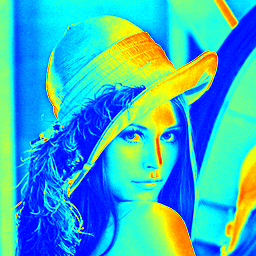
\includegraphics[width=0.3\textwidth]{imagenes/lenaTEMP.jpg}
\end{wrapfigure}

El filtro temperatura toma una imagen fuente y genera un efecto que simula un mapa de calor. Dicho efecto lo consigue tomando los tres componentes de color de cada pixel y promediándolos. Luego le asigna un valor que depende de este promedio \textit{t}.

\begin{center}
$\mathsf{t}_{(i,j)} = \lfloor(\mathsf{src}.r_{(i,j)} + \mathsf{src}.g_{(i,j)} + \mathsf{src}.b_{(i,j)}) / 3\rfloor$
\end{center}

Finalmente el color en la imagen destino se determina en función de la temperatura \textit{t} conforme al siguiente mapeo:

\begin{center}
\begin{displaymath}
\mathsf{dst}_{(i,j)}<r,g,b> = \left\{
\begin{array}{l l}
			<0,0, 128 + t \cdot 4> & \text{si }t < 32\\
			<0, (t - 32) \cdot 4, 255> & \text{si }32 \le t < 96\\
			<(t-96) \cdot 4, 255, 255 - (t-96) \cdot 4> & \text{si }96 \le t < 160\\
			<255, 255 - (t - 160) \cdot 4, 0> & \text{si }160 \le t < 224\\
			<255 - (t - 224) \cdot 4, 0 , 0> & \text{si no} \\
\end{array}
\right.
\end{displaymath}
\end{center}

\hfill
\subsubsection{Implementación C}

El algoritmo implementado en lenguaje C recorre la imagen iterativamente. Por cada pixel en la imagen original calcula el promedio de sus componentes RGB (línea 4) y según este valor se guarda en la imagen destino el calculo correspondiente a la temperatura (líneas 5 a 15). A continuación el pseudocódigo:
	
\begin{algorithm}[H]
  \begin{algorithmic}[1]
		\FORALL{y:=0 \TO  Height($I_{src}$)}
			\FORALL{x:=0 \TO  Width($I_{src}$)}
				\STATE $ pixel \gets I_{src}(x,y)$
				\STATE $Nat $ $ t \gets \lfloor(\frac{Red(pixel)+Green(pixel)+Blue(pixel)}{3}\rfloor$
				\IF{$t < 32$}
					\STATE $I_{dst}(x,y) \gets DevolverPixel(0,0,128+t \cdot 4)$
				\ELSIF{$ 32 \leq t < 96$}
					\STATE $I_{dst}(x,y) \gets DevolverPixel(0,(t-32) \cdot 4,255)$
				\ELSIF{$ 96 \leq t < 160$}
					\STATE $I_{dst}(x,y) \gets DevolverPixel((t-96) \cdot 4,255, 255-(t-96) \cdot 4)$
				\ELSIF{$ 160 \leq t < 224$}
					\STATE $I_{dst}(x,y) \gets DevolverPixel(255, 255-(t-160) \cdot 4, 0)$
				\ELSE		
					\STATE $I_{dst}(x,y) \gets DevolverPixel(255-(t-224) \cdot 4, 0, 0)$
				\ENDIF	
			\ENDFOR
		 \ENDFOR
  \end{algorithmic}
  \caption{$temperature (I_{src}, I_{dst})$}
  \label{alg:temperature}
\end{algorithm}	

\subsubsection{Implementación ASM}